\chapter{Designing the Dataset}
\label{ch:dataset-design}

\emph{Opening dilemma.} A team builds a pedestrian detector for a campus shuttle. The validation accuracy on their training distribution is excellent. The first week of live operation, the system misses every pedestrian at dusk on the elm-lined approach to the dining hall. The team's instinct is to label more data: thousands of additional frames are queued for annotation. A skeptical engineer asks the awkward question: is ``more data'' the right answer, or did the team's earlier choice to label only midday footage already decide what the model would never learn? The labeled set was the model's entire experience of the world. The dataset was a design choice; the team just did not notice they were designing.

Earlier chapters framed the learning problem, chose metrics, protected evaluation, and diagnosed structural gaps. One critical question stayed deferred: how should the training data itself be designed? Data is a design choice, not a given. The same task can be tackled with different examples, different labeling schemes, different class distributions, and different label-quality standards. Each choice changes what the model can learn and how it behaves in the world.

This chapter treats dataset construction as a modeling decision, not preprocessing. Who labels the data? What counts as a valid label when annotators disagree? How should class imbalance be handled? When should a team invest in more examples, cleaner labels, or better-curated examples? When labels are expensive, which examples should be labeled next? When does synthetic data help, and when does it mislead? Each answer shapes the learning problem itself.

By the end of this chapter, you should be able to state what data-design choices your task requires, defend them on grounds of coverage and quality, and build a data design card that records the assumptions baked into the dataset.

\begin{practicalnote}
\textbf{Core path.} The required path covers label definition, annotator consistency, label noise, class balance, coverage, and the data design card. Active learning, semi-supervised learning, weak supervision, augmentation, and synthetic data are label-acquisition strategies. Assign them selectively or treat them as extensions once the core data-design decisions are stable.
\end{practicalnote}

Data design is not optional cleanup before real modeling begins. It is part of the model. The examples labeled, the labels themselves, and their distribution are deliberate design choices that constrain what the model can learn and where it will fail.

\textbf{Data as design.} When evaluating a model, always ask three questions. What does the dataset tell the model is important? What structure or distribution is missing from the training set? What gaps exist between the labeled data and the deployment population?

\begin{decisionbox}
\textbf{Data-design order of operations.} Do not start with augmentation, synthetic data, or a larger labeling budget. First define what each label means and who may assign it. Then measure label quality and disagreement. Next compare the data distribution with the deployment distribution and the operating policy. Only after those checks should the team pick a label-acquisition strategy such as active learning, semi-supervised learning, weak supervision, augmentation, or synthetic data.
\end{decisionbox}

\section{Data as a Design Decision}

The dataset encodes assumptions about the world. What you include, exclude, label, and measure shapes the model as much as the architecture does. A model trained only on examples from September through November will never see winter-specific behavior. A student-support system trained on cases labeled by one kind of advisor learns a different definition of ``risk'' than one trained on cases labeled by advisors with different philosophies. A pedestrian detector trained only on sunny weather will fail at dusk.

These are not minor problems to be patched later through validation. They are fundamental limits on what the model can learn.

\subsection{Two Running Cases}

Keep two settings in view throughout this chapter. Both appeared earlier; here they become frameworks for data-design decisions.

\textbf{Case 1: Course-Support Assistant.} A university builds an early-warning system to flag students who may need extra support. The system needs labeled historical data. Which messages get labeled? Does every submission receive a label, or only high-uncertainty ones? Do labels come from a single trained expert advisor, or from multiple advisors with different standards? If two advisors disagree about whether a message signals ``urgent need for support,'' is that disagreement noise or information? The answer shapes both the dataset and the model.

\textbf{Case 2: Pedestrian Detector.} A campus shuttle system uses computer vision to detect pedestrians. The model needs labeled video frames. Which frames belong in the training set? Only clear daylight footage, or also dawn, dusk, and night? All weather conditions? Which camera angles? And what about occlusions---should a partially visible pedestrian count as present or absent? These choices determine what the model learns about pedestrian detection.

In both cases, someone must decide what examples matter, how to label them, and what quality standard to enforce. These are dataset-design decisions, not cleanup tasks.

\begin{figure}[t]
\centering
\definecolor{c4bdataInclude}{RGB}{210,238,220}
\definecolor{c4bdataExclude}{RGB}{254,216,216}
\definecolor{c4bdataLabel}{RGB}{220,233,251}
\resizebox{\linewidth}{!}{%
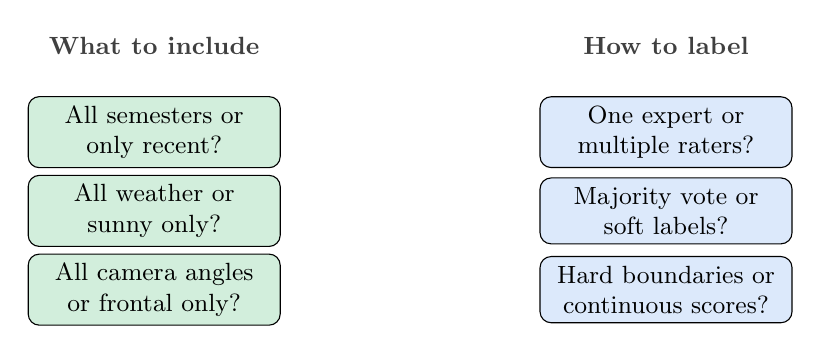
\begin{tikzpicture}[x=1cm, y=1cm, font=\small]
%% Panel A: what examples to include
\begin{scope}
  \node[font=\small\bfseries, black!75] at (2.0, 4.0) {What to include};
  \node[draw, fill=c4bdataInclude, rounded corners, align=center,
        minimum height=0.7cm, minimum width=3.2cm]
    at (2.0, 2.9) {All semesters or\\only recent?};
  \node[draw, fill=c4bdataInclude, rounded corners, align=center,
        minimum height=0.7cm, minimum width=3.2cm]
    at (2.0, 1.9) {All weather or\\sunny only?};
  \node[draw, fill=c4bdataInclude, rounded corners, align=center,
        minimum height=0.7cm, minimum width=3.2cm]
    at (2.0, 0.9) {All camera angles\\or frontal only?};
\end{scope}
%% Panel B: labeling choices
\begin{scope}[xshift=6.5cm]
  \node[font=\small\bfseries, black!75] at (2.0, 4.0) {How to label};
  \node[draw, fill=c4bdataLabel, rounded corners, align=center,
        minimum height=0.7cm, minimum width=3.2cm]
    at (2.0, 2.9) {One expert or\\multiple raters?};
  \node[draw, fill=c4bdataLabel, rounded corners, align=center,
        minimum height=0.7cm, minimum width=3.2cm]
    at (2.0, 1.9) {Majority vote or\\soft labels?};
  \node[draw, fill=c4bdataLabel, rounded corners, align=center,
        minimum height=0.7cm, minimum width=3.2cm]
    at (2.0, 0.9) {Hard boundaries or\\continuous scores?};
\end{scope}
\end{tikzpicture}%
}
\caption{Data design has two main dimensions: which examples to collect and how to label them. Each choice affects what the model learns.}
\label{fig:data-design-dimensions}
\end{figure}

\section{Annotation Protocols and Label Quality}

Collecting labels is not as simple as hiring someone to point and click. The labeling process is itself a design decision.

\subsection{Annotation Guidelines and Consistency}

The first step is to write clear annotation guidelines. Good guidelines specify:
\begin{itemize}[leftmargin=*]
\item What examples should be labeled and which should be skipped
\item What each label means and what behavior or feature it identifies
\item How to handle edge cases and borderline examples
\item How to resolve ambiguity
\end{itemize}

For the course-support system, a guideline might say:

\begin{codeexample}[caption={Sample annotation guideline for student messages}]
Label URGENT if:
- Student mentions missing deadline or financial hardship
- Student indicates suicidal ideation or severe mental health crisis
- Student reports discrimination or safety concern

Label CONCERNING if:
- Multiple late submissions in one week
- Sudden drop in engagement or attendance
- Student reports confusion about course mechanics

Label ROUTINE otherwise
\end{codeexample}

\begin{warningbox}
High-stakes student-support labels are not only an annotation problem. A dataset that contains mental-health crisis, discrimination, financial hardship, demographics, advising notes, or learning-management-system records also needs governance rules: consent or a lawful institutional basis, data minimization, restricted access, escalation protocols, human review, and a clear statement that the model output is not a welfare decision. Label quality cannot substitute for those safeguards.
\end{warningbox}

Good guidelines reduce annotator variation and make labeling reproducible. They cannot eliminate disagreement entirely.

\subsection{Inter-Annotator Agreement and Soft Labels}
\label{sec:soft-labels}

When multiple annotators label the same example, they often disagree. Practitioners usually treat this disagreement as noise, but sometimes it carries information. When two trained advisors disagree about whether a student message indicates ``urgent'' need, the disagreement often reflects genuine ambiguity in the task rather than one ``right answer'' that one rater found and the other missed.

\begin{definition}[Inter-Annotator Agreement]
Inter-annotator agreement is the degree to which independent annotators assign the same labels to the same examples, typically measured by Cohen's kappa, Fleiss's kappa, or Krippendorff's alpha.
\end{definition}

\textbf{Cohen's kappa.} For two annotators labeling the same examples, let $p_o$ be the observed proportion of agreements and $p_e$ the proportion expected by chance under each annotator's marginal label frequencies. Cohen's kappa is
\[
\kappa = \frac{p_o - p_e}{1 - p_e}.
\]
Values near $1$ indicate strong agreement beyond chance; $0$ means agreement at the chance level; negative values indicate systematic disagreement. Fleiss's kappa generalizes to more than two annotators; Krippendorff's alpha further allows ordinal or interval labels and missing values.

Low agreement signals one of three things: unclear guidelines, an inherently ambiguous task, or undertrained annotators. Each is worth investigating before treating disagreement as noise to be averaged away.

Three common strategies exist.

\textbf{Majority vote.} Give each example to multiple raters and assign the label that most raters chose. This works well when agreement is high and annotators are reasonably reliable, but it discards disagreement information and is brittle to systematic annotator bias.

\textbf{Adjudication.} Send disagreed-upon examples to a senior expert who makes the final call. This handles edge cases well but creates a single-expert bottleneck and does not capture underlying ambiguity.

\textbf{Soft labels.} Record the fraction of annotators who chose each label. Instead of a single ``URGENT'' or ``ROUTINE'' label, record that 0.7 of raters chose URGENT and 0.3 chose ROUTINE. This preserves disagreement and lets models learn that some examples are genuinely uncertain.

\begin{example}[Soft Labels for Student Messages]
Two advisors each label ten student messages. On one message about a missed assignment, one advisor chooses CONCERNING and the other chooses ROUTINE. Majority vote forces an arbitrary hard label. Soft labels record $[0.5, 0.5]$, capturing the genuine ambiguity. A model trained on soft labels learns to output moderate confidence on similar cases instead of being forced to pick a side.
\end{example}

For short guidelines and tasks that feel objective (``does this image contain a car?''), majority vote is usually enough. For long guidelines and subjective or ambiguous tasks (``is this message urgent?''), soft labels or adjudication preserve more information. Measure inter-annotator agreement before committing to one strategy.

\section{Label Noise and Its Effects}
\label{sec:label-noise}

Labels are often imperfect. Noise can be random, or it can be systematic---for example, one annotator consistently mislabels a particular class. The effect of label noise varies significantly across models.

\subsection{Types of Label Noise}

\begin{definition}[Symmetric Noise]
Symmetric label noise flips each label to a random wrong label with equal probability. A positive example becomes negative with probability $p$, and vice versa, randomly.
\end{definition}

\begin{definition}[Asymmetric Noise]
Asymmetric label noise has a preferred direction. For example, positive examples might be mislabeled as negative 10\% of the time, while negative examples are mislabeled as positive only 2\% of the time. This often reflects annotator bias or systematic confusion.
\end{definition}

\subsection{Noise Robustness Across Model Families}

Different model families tolerate label noise differently.

\textbf{Decision trees.} Trees handle small amounts of random label noise reasonably well because they partition the input space and make local decisions. Noise in one region does not necessarily affect splits in another. Trees can still overfit to noise, especially at deep depths.

\textbf{Linear models.} Linear models are sensitive to label noise because each training example contributes directly to the gradient and the final coefficients. Outliers and mislabeled examples are felt globally.

\textbf{Neural networks.} Neural networks are sensitive to label noise early in training but, with enough capacity, eventually memorize noisy labels. The memorization looks like overfitting: the model fits the noise perfectly on the training set but generalizes poorly.

No model is immune to noise. The real question is which kind of noise your model can afford and whether the right response is cleaning labels or switching to noise-robust losses.

\begin{warningbox}
Systematic mislabeling is much worse than random noise. If all positive examples of a particular type are mislabeled as negative because of annotator confusion, the model learns the wrong boundary in that region. Random noise averages out to some degree; systematic noise teaches the wrong pattern.
\end{warningbox}

\subsection{Label-Noise Strategies}

When labels are noisy, several strategies exist.

\textbf{Clean the labels.} Have a senior expert audit and correct a sample of labels. Expensive, but effective when noise is mostly systematic.

\textbf{Use noise-aware training.} Some training procedures reduce the influence of suspected label errors. A team might estimate class-conditional noise rates and correct the loss, down-weight examples whose labels strongly contradict a clean validation signal, or use robust losses designed for noisy labels. Be careful with focal loss: it is primarily a class-imbalance and hard-example weighting tool, and on its own it can amplify attention to mislabeled hard cases.

\textbf{Estimate noise rates.} If you can estimate how often each class is mislabeled, you can adjust the loss function accordingly. This requires a clean validation set or a held-out sample for the estimate.

\textbf{Threshold and filter.} Train the model and remove or down-weight examples the model is highly confident were mislabeled---those where its prediction strongly contradicts the given label.

Northcutt et al.\ found widespread label errors across common benchmark test sets---averaging at least 3.3\% across ten datasets---and showed that corrected labels can change which model appears best \citep{northcutt2021labelerrors}. Related confident-learning work shows how systematic label auditing can identify likely errors and improve downstream training \citep{northcutt2021confidentlearning}. Cleaning important datasets is not busy work; it can directly change the evidence used to judge trained models.

\begin{advancednote}
\textbf{When does training on noisy labels still recover the right classifier?} Natarajan et al.\ 2013 give a precise answer for binary classification under class-conditional noise. Let $\rho_+$ be the probability that a true positive label is flipped to negative and $\rho_-$ the probability that a true negative is flipped to positive, and assume $\rho_+ + \rho_- < 1$. For any standard convex surrogate loss $\ell(\hat y, y)$ used on clean labels, the corrected loss
\[
\tilde\ell(\hat y, y) = \frac{(1 - \rho_{-y})\,\ell(\hat y, y) - \rho_y\,\ell(\hat y, -y)}{1 - \rho_+ - \rho_-}
\]
is an unbiased estimator of the clean loss in the sense that $\mathbb{E}_{\tilde y \mid y}[\tilde\ell(\hat y, \tilde y)] = \ell(\hat y, y)$, where $\tilde y$ denotes the observed (possibly flipped) label. Empirical risk minimization with $\tilde\ell$ on the \emph{noisy} data is therefore consistent for the clean Bayes-optimal classifier.

Operationally, the result says that if the noise rates $\rho_+, \rho_-$ can be estimated---typically from a small clean validation set or a held-out audit---there is no need to clean the training data before fitting; an unbiased classifier can be trained directly on the noisy labels with the corrected loss. This is the theoretical foundation underneath ``confident learning'' and Cleanlab-style methods: the confident-learning estimator of Northcutt et al.\ \citep{northcutt2021confidentlearning} cited above is one practical way to estimate the flip rates $\rho_+, \rho_-$ that the correction formula requires. The limit is sharp: when $\rho_+ + \rho_- \geq 1$ the labels are no more informative than coin flips, the denominator in $\tilde\ell$ collapses, and no consistent estimator of the clean Bayes classifier exists from the noisy data alone.
\end{advancednote}

\textbf{Noise investigation.} When validation performance is worse than expected, ask whether label noise is the culprit before blaming the model. Sample and hand-inspect a small random subset of training labels to estimate noise rates.

\section{Class Imbalance: Problem or Design Choice?}

The most common advice about class imbalance is to ``balance the classes.'' That is usually wrong. The right question is what the deployment distribution looks like.

\begin{definition}[Class Imbalance]
Class imbalance occurs when one class appears much more frequently than another in the training set. A 95--5 split is heavily imbalanced; a 60--40 split is mildly imbalanced.
\end{definition}

The default worry is that the model will learn to predict the majority class and ignore the minority. That risk is real if you evaluate on a metric like accuracy, which the majority class dominates. But the problem is not inherent to imbalanced data; it is a problem of evaluation and loss design.

\subsection{Imbalance in Context}

If deployment is also 95--5 (95\% negative, 5\% positive), training on a 95--5 distribution is appropriate. The model should predict the majority class frequently, just as deployment requires.

If deployment is 50--50, training on a 95--5 distribution is a distribution-mismatch problem. The model sees too few minority examples to learn rich decision boundaries for the deployment setting. Separately, if the minority class matters more than its prevalence suggests, reflect that through class weights, decision thresholds, and evaluation metrics rather than by pretending the deployment prevalence is different.

\subsection{Addressing Imbalance}

When the training distribution does not match the deployment distribution, several strategies exist.

\textbf{Oversampling the minority class.} Duplicate minority examples or generate similar ones until the classes are balanced. This increases the influence of minority examples but risks overfitting, since the model sees the same minority examples many times.

\textbf{Undersampling the majority class.} Remove majority examples until the classes are balanced. This discards potentially informative examples and works only when majority data is so abundant that removal is inconsequential.

\textbf{Class-weighted loss.} Give minority examples a higher loss weight so an error on a minority example costs more than an error on a majority example. Computationally efficient and preserves all the data, but it makes implicit assumptions about deployment importance.

\textbf{Threshold adjustment.} Train on the original imbalanced distribution and adjust the decision threshold to reflect the deployment distribution. Effective when the model outputs a well-calibrated score, but requires knowing the deployment and score distributions in advance.

\begin{decisionbox}
\textbf{When to balance the classes:}
\begin{itemize}
\item Training and deployment distributions differ, and the minority class matters operationally.
\item You need the model to learn rich decision boundaries for both classes.
\item You care equally about minority and majority recall, or you want a balanced F1 score.
\end{itemize}
\textbf{When to keep the imbalance:}
\begin{itemize}
\item Training and deployment distributions match (both imbalanced the same way).
\item Class importance and error costs are intended to follow the deployment distribution.
\item You evaluate with metrics appropriate for imbalance, such as PR-AUC, macro-F1, balanced accuracy, or cost-sensitive utility; ROC-AUC can help but is not sufficient on its own under extreme imbalance.
\end{itemize}
\end{decisionbox}

\begin{example}[Imbalance in Pedestrian Detection]
A campus shuttle's pedestrian detector is trained on all video frames collected during data gathering. 99\% of frames contain no pedestrians; only 1\% do. If the deployment camera sees a similar 99--1 split because pedestrians really are rare, training on that distribution is fine: the model should predict ``no pedestrian'' most of the time. But if the model is deployed in times and places where pedestrians are more common---outside a busy building, say---the 99--1 training distribution becomes misleading and the model grows too conservative about detecting pedestrians. Reweighting or threshold adjustment is appropriate in that scenario.
\end{example}

\section{More Data, Better Data, or Better Labels?}

Data-centric ML holds that modeling progress often comes not from better algorithms but from better data. The practical question follows: should a team invest limited resources in collecting more examples, cleaning existing examples, or improving label quality?

\subsection{When More Data Helps}

More data helps most when:
\begin{itemize}[leftmargin=*]
\item The current model exhibits high variance: training error is low but validation error is high
\item The current dataset does not cover the full diversity of the deployment population
\item The task is well-defined, labels are reliable, and the bottleneck is lack of examples
\end{itemize}

More random examples help least when label noise is the main problem or when the data distribution is far from deployment.

\subsection{When Better Labels Help}

Better labels matter most when:
\begin{itemize}[leftmargin=*]
\item Label noise is high: multiple validation samples show disagreement or suspicious labels
\item Both training and validation error are high, and inspection suggests label ambiguity or systematic label errors
\item Annotation guidelines are unclear or inconsistently applied
\end{itemize}

Cleaning and improving labels is often cheaper than collecting more examples and can deliver immediate performance gains.

\subsection{When Better Coverage Helps}

Better coverage or data augmentation helps most when:
\begin{itemize}[leftmargin=*]
\item The training distribution has systematic gaps (e.g., no night-time pedestrian frames)
\item The model systematically fails on a slice of the deployment data (e.g., very crowded scenes)
\item Existing examples are not diverse enough to train the model on the true variation in the deployment environment
\end{itemize}

\begin{figure}[t]
\centering
\definecolor{c4bvarianceColor}{RGB}{56,103,170}
\definecolor{c4bbiasColor}{RGB}{180,40,40}
\definecolor{c4bnoisColor}{RGB}{184,92,16}
\resizebox{\linewidth}{!}{%
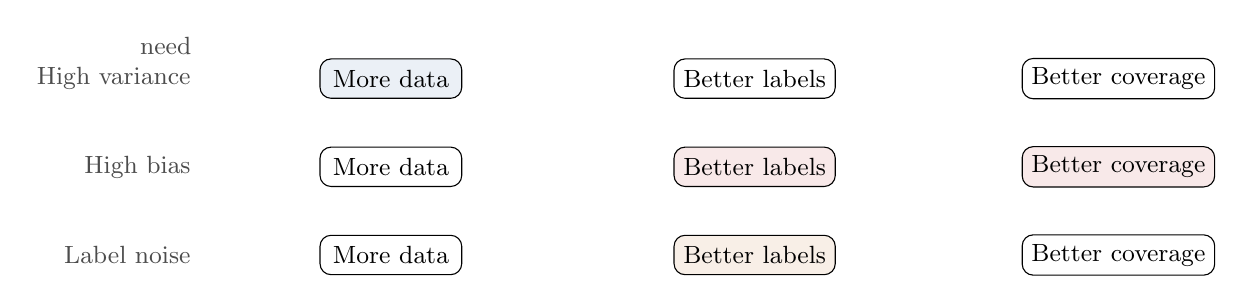
\begin{tikzpicture}[x=2.2cm, y=1.4cm, font=\small]
%% Axis labels
\node[black!70, font=\small] at (-0.4, 2.3) {need};
%% Row 1: High variance (more data helps)
\node[anchor=east, black!70, font=\small] at (-0.2, 2.0) {High variance};
\node[draw, fill=c4bvarianceColor!10, rounded corners, align=center,
      minimum height=0.5cm, minimum width=1.8cm]
  at (0.9, 2.0) {More data};
\node[draw, fill=white, rounded corners, align=center,
      minimum height=0.5cm, minimum width=1.8cm]
  at (3.0, 2.0) {Better labels};
\node[draw, fill=white, rounded corners, align=center,
      minimum height=0.5cm, minimum width=1.8cm]
  at (5.1, 2.0) {Better coverage};
%% Row 2: High bias (better labels or coverage helps)
\node[anchor=east, black!70, font=\small] at (-0.2, 1.2) {High bias};
\node[draw, fill=white, rounded corners, align=center,
      minimum height=0.5cm, minimum width=1.8cm]
  at (0.9, 1.2) {More data};
\node[draw, fill=c4bbiasColor!10, rounded corners, align=center,
      minimum height=0.5cm, minimum width=1.8cm]
  at (3.0, 1.2) {Better labels};
\node[draw, fill=c4bbiasColor!10, rounded corners, align=center,
      minimum height=0.5cm, minimum width=1.8cm]
  at (5.1, 1.2) {Better coverage};
%% Row 3: Label noise (better labels helps)
\node[anchor=east, black!70, font=\small] at (-0.2, 0.4) {Label noise};
\node[draw, fill=white, rounded corners, align=center,
      minimum height=0.5cm, minimum width=1.8cm]
  at (0.9, 0.4) {More data};
\node[draw, fill=c4bnoisColor!10, rounded corners, align=center,
      minimum height=0.5cm, minimum width=1.8cm]
  at (3.0, 0.4) {Better labels};
\node[draw, fill=white, rounded corners, align=center,
      minimum height=0.5cm, minimum width=1.8cm]
  at (5.1, 0.4) {Better coverage};
\end{tikzpicture}%
}
\caption{Data investment decisions should depend on whether the bottleneck is variance (too few examples), bias (gaps in coverage), or noise (unreliable labels).}
\label{fig:data-investment-choice}
\end{figure}

\textbf{Data investment triage.} Before collecting new data, diagnose the failure mode. If training error is much lower than validation error, the problem is variance. If both are high, the problem is bias or coverage. If labels look unreliable, the problem is noise. Invest accordingly.

\section{Active Learning: Labeling Strategically}

When labeling is expensive---because it requires expert annotation or manual review---labeling every available example is wasteful. Active learning asks which examples to label next to improve the model most.

\subsection{Core Active Learning Strategies}

\textbf{Uncertainty sampling.} Label the examples for which the current model is least confident. For a probabilistic classifier, this means examples where the predicted probability is closest to 0.5 (binary) or most spread across classes. The model has already learned what it can from confident examples; uncertain ones carry more information.

\textbf{Diversity sampling.} Label examples that are most different from those already labeled, measured through clustering, embedding distance, or other diversity metrics. Diversity prevents the model from learning only about clusters of similar examples.

\textbf{Expected model change.} Estimate how much labeling each unlabeled example would shift the model parameters if it were labeled and the model retrained. Label the examples with the highest expected change. This requires training multiple candidate models or estimating gradient impact.

\subsection{When Active Learning Pays Off}

Active learning is most valuable when:
\begin{itemize}[leftmargin=*]
\item Labeling is genuinely expensive (requires expert time, not just crowdsourcing)
\item You have a large pool of unlabeled examples
\item The model's uncertainty is informative (it reflects genuine task difficulty, not just poor calibration)
\item You have time to iterate: label a batch, retrain, select the next batch
\end{itemize}

Active learning is least useful when labeling is cheap, the unlabeled pool is small, or the model is poorly calibrated.

\begin{example}[Active Learning for Course Support]
A university starts with 100 randomly labeled student messages. The early-warning model performs reasonably but has room to improve. Instead of randomly labeling 100 more messages, the team uses uncertainty sampling: they ask the model for the 100 unlabeled messages where it is least confident. A domain expert (student advisor) labels only those 100. With 200 total labels---100 of them strategically chosen---the model improves more than it would from 200 random labels. The team gets more improvement from the same expert time by skipping examples the model already handles confidently.
\end{example}

Active learning requires discipline. The model must be retrained after each labeling round, and the uncertainty estimates must be reliable. An overconfident or poorly calibrated model will steer uncertainty sampling toward uninformative examples. Test active learning on a small batch first before committing to a full labeling campaign.

\section{Learning with Fewer Labels (Extension)}
\label{sec:fewer-labels}

Active learning asks \emph{which} examples to label next. A different question is often more pressing: can the model learn from examples that have no labels at all, or from labels that are noisy and automatically generated? In many real-world settings, unlabeled data is abundant and labeled data is scarce. A university's learning management system may contain hundreds of thousands of student messages, but only a few hundred reviewed by an advisor. A campus shuttle may record millions of video frames, but only a small fraction have bounding boxes. The gap between available data and labeled data is the central problem of this section.

Two families of techniques address that gap. \emph{Semi-supervised learning} uses the structure of unlabeled data to improve a model trained on a small labeled set. \emph{Weak supervision} replaces expensive human labels with cheaper, noisier labels produced by rules, heuristics, or external knowledge sources. Both extend the chapter's core argument: data is a design choice, and the label-acquisition strategy is part of that design.

\subsection{Semi-Supervised Learning}

Semi-supervised learning exploits a simple insight: even without labels, the distribution of the input data carries information about the structure of the problem. Clusters, manifolds, and density patterns in unlabeled data can guide the model toward better decision boundaries.

\subsubsection{Self-Training}

Self-training is the simplest semi-supervised method:

\begin{enumerate}[leftmargin=*]
\item Train a model on the small labeled dataset.
\item Use the trained model to predict labels for the unlabeled examples.
\item Select the predictions where the model is most confident (above some threshold).
\item Add those examples, with their predicted labels, to the training set.
\item Retrain the model on the expanded training set.
\item Repeat until no more confident predictions remain or performance stops improving.
\end{enumerate}

The predicted labels assigned in step 3 are called \emph{pseudo-labels}. They are not ground truth---they are the model's best guesses, treated as if they were real labels.

\begin{example}[Self-Training for Course Support]
A university has 200 labeled student messages and 10{,}000 unlabeled ones. The team trains an initial classifier on the 200 labeled messages, then predicts labels for all 10{,}000 unlabeled messages. For the 1{,}200 messages where confidence exceeds 0.95, the predicted labels become pseudo-labels and join the training set. The model retrains on the expanded set of 1{,}400 examples. The process repeats, adding a few hundred more high-confidence pseudo-labels each round. After three rounds, the model has effectively used 2{,}800 examples despite only 200 having real human labels.
\end{example}

\begin{warningbox}
Self-training amplifies the model's existing biases. If the initial model misclassifies a cluster---say, formal but urgent student messages as ROUTINE because they lack emotional language---self-training confidently assigns ROUTINE pseudo-labels to similar messages, reinforcing the error. This is \emph{confirmation bias} in self-training. Monitor pseudo-label quality by spot-checking a random sample and tracking performance on a held-out validation set after each round.
\end{warningbox}

\subsubsection{Co-Training}

\begin{advancednote}
Co-training addresses self-training's confirmation bias by using two models instead of one. The idea requires two \emph{views} of the data---two feature sets that are each sufficient for the task but provide complementary information.

Each model trains on the labeled data using its own view. Each then labels the unlabeled examples, and the most confident predictions from \emph{one} model join the training set of the \emph{other}. Because the two models see different features, they make different errors, and each corrects the other.

\begin{example}[Co-Training for Pedestrian Detection]
A pedestrian detection system has two views: visual appearance (image pixels) and motion patterns (optical flow between consecutive frames). Model A learns from appearance; Model B learns from motion. Model A confidently identifies a stationary person at a crosswalk---easy to see in the image but invisible to motion. Model B confidently identifies a jogger in a cluttered background---hard to see in a single frame but obvious from motion. Each model's confident predictions become training data for the other, expanding what both can detect.
\end{example}

The co-training requirement for two independent, sufficient views is rarely met perfectly in practice. Common relaxations include using two different architectures on the same features, or random feature splits. These approximations often help, but the theoretical guarantees weaken. If your features do not naturally split into two independent views, self-training or the weak supervision methods below may be more practical.
\end{advancednote}

\subsection{Pseudo-Label Quality and the Confidence Threshold}

The success of every pseudo-labeling method depends on pseudo-label quality. Two design decisions control that quality.

\textbf{Confidence threshold.} A higher threshold (say, 0.99) produces fewer but more reliable pseudo-labels. A lower one (say, 0.8) produces more pseudo-labels and more noise. The right threshold trades the cost of a wrong pseudo-label against the benefit of more training data.

\textbf{Curriculum strategy.} Rather than fixing a threshold, some methods start high and gradually lower it across rounds. This \emph{curriculum} approach adds the easiest examples first, building a stronger model before tackling ambiguous cases.

\begin{decisionbox}
\textbf{Semi-supervised method selection:}
\begin{itemize}
\item With one feature set and a simple pipeline, start with self-training. It is the easiest to implement and debug.
\item With two naturally complementary views of the data (text and metadata, image and motion), consider co-training.
\item In all cases, monitor pseudo-label quality: spot-check a sample, track validation performance after each round, and stop if performance degrades.
\item Combine with active learning: expand the training set cheaply through semi-supervised methods, then use active learning to select the most valuable examples for expensive human labeling.
\end{itemize}
\end{decisionbox}

\subsection{Weak Supervision}
\label{subsec:weak-supervision}

Semi-supervised learning extracts signal from \emph{unlabeled} data. Weak supervision takes a different route: it generates labels automatically using heuristics, rules, and external knowledge. These labels are noisier than expert annotations, but they can be produced at scale and at near-zero marginal cost.

\subsubsection{Labeling Functions}

The core building block of weak supervision is the \emph{labeling function}: a simple rule or heuristic that assigns a label based on an observable pattern. A labeling function does not need to be accurate on all examples; it only needs to be informative on the examples it chooses to label.

\begin{example}[Labeling Functions for Course Support]
A team building the student early-warning system writes several labeling functions:
\begin{itemize}[leftmargin=*]
\item \texttt{lf\_keyword\_urgent}: if the message contains ``crisis,'' ``emergency,'' or ``suicide,'' label URGENT
\item \texttt{lf\_late\_submissions}: if the student has 3+ late submissions this week, label CONCERNING
\item \texttt{lf\_engagement\_drop}: if the student's login frequency dropped by more than 50\% compared to the previous two weeks, label CONCERNING
\item \texttt{lf\_routine\_length}: if the message is fewer than 10 words and contains a question mark, label ROUTINE
\end{itemize}
Each labeling function covers only a subset of examples and may abstain (assign no label) on most of the data. Each one encodes domain knowledge that would otherwise require expert annotation.
\end{example}

\subsubsection{Data Programming: Combining Labeling Functions}

\begin{advancednote}
Individual labeling functions are noisy and incomplete. The insight of \emph{data programming} is to combine many of them into a single, higher-quality label estimate. The framework, developed in the Snorkel system, works as follows:

\begin{enumerate}[leftmargin=*]
\item Write multiple labeling functions, each capturing a different heuristic or knowledge source.
\item Apply all labeling functions to the unlabeled data. Each example may receive labels from several functions, one function, or none.
\item Use a \emph{label model} to estimate the accuracy and correlation structure of the labeling functions \emph{without any ground-truth labels}. The label model treats each labeling function as a noisy voter and infers the most likely true label by modeling agreement and disagreement patterns.
\item Use the label model's probabilistic output as training labels for a downstream model.
\end{enumerate}

The label model is the critical component. It learns which labeling functions are accurate, which are correlated (and so provide redundant signal), and which disagree in informative ways. The output is a probabilistic (soft) label for each example, usable directly as a training target.
\end{advancednote}

Writing labeling functions is a way to encode domain knowledge. The quality of weak supervision depends on how much relevant knowledge you can express as simple rules. Start by interviewing domain experts: ``What patterns do you look for when labeling this task?'' Each answer is a candidate labeling function. Aim for 10--30 labeling functions with diverse coverage; a few high-precision functions (rarely wrong, often abstain) are more valuable than many low-precision ones.

\begin{warningbox}
Correlated labeling functions treated as independent will cause the label model to overcount their shared signal. If three functions all check for keyword overlap with the same word list, the label model may treat their agreement as strong evidence when it is really one signal counted three times. Audit your labeling functions for correlation before training the label model.
\end{warningbox}

\subsubsection{Silver Labels: Terminology and Trust}

Labels produced by labeling functions or label models are sometimes called \emph{silver labels}, to distinguish them from expert-annotated \emph{gold labels}. Silver labels are cheaper but noisier.

The critical design question is how much to trust silver labels. Three strategies are common.

\begin{itemize}[leftmargin=*]
\item \emph{Train on silver, evaluate on gold.} Use silver labels for training, but always evaluate on a small set of expert-annotated gold labels. This is the minimum standard: without gold evaluation, you cannot measure how much noise the silver labels introduce.
\item \emph{Weight by confidence.} If the label model produces probabilistic outputs, weight training examples by its confidence. High-confidence silver labels contribute more to the loss; low-confidence ones contribute less. This is analogous to soft labels from annotator disagreement (Section~\ref{sec:soft-labels}).
\item \emph{Mix gold and silver.} Combine gold labels (expensive, small) with silver labels (cheap, large). Gold labels anchor the model; silver labels provide coverage. The mixing ratio is a hyperparameter: too little gold and the model trusts noisy silver labels; too much and the silver labels add nothing.
\end{itemize}

\begin{example}[Weak Supervision for Pedestrian-Presence Classification]
A pedestrian-analytics team has 500 expert-labeled frames (gold) indicating whether each frame contains at least one pedestrian, plus 50{,}000 additional unlabeled frames from campus cameras. They write labeling functions using motion detection (moving objects above a certain size are likely pedestrians), time-of-day priors (frames captured during class changes are more likely to contain pedestrians), and a pretrained generic object detector (whose ``person'' predictions are a noisy vote on pedestrian presence). A label model combines these three sources into probabilistic silver labels. The team trains a frame-level classifier on 500 gold frames plus 50{,}000 silver-labeled frames, evaluates on a held-out set of 200 gold frames, and finds the silver-augmented model beats the gold-only model by 8 percentage points on recall, detecting more pedestrian-present frames in difficult conditions (dusk, rain) where the gold training set had few examples.
\end{example}

\subsection{Connecting the Pieces}

Active learning, semi-supervised learning, and weak supervision are not competing strategies. They are complementary tools in a label-acquisition \emph{pipeline}. A practical workflow might proceed as follows:

\begin{enumerate}[leftmargin=*]
\item Start with a small labeled seed set (gold labels).
\item Use weak supervision to generate silver labels for a large unlabeled pool.
\item Train an initial model on gold + silver labels.
\item Use active learning to select the most valuable examples from the remaining unlabeled pool for expert annotation.
\item Use semi-supervised self-training to propagate labels to confident unlabeled examples.
\item Repeat: each round adds a mix of gold labels (from active learning), silver labels (from labeling functions), and pseudo-labels (from self-training).
\end{enumerate}

\begin{figure}[t]
\centering
\resizebox{0.85\linewidth}{!}{%
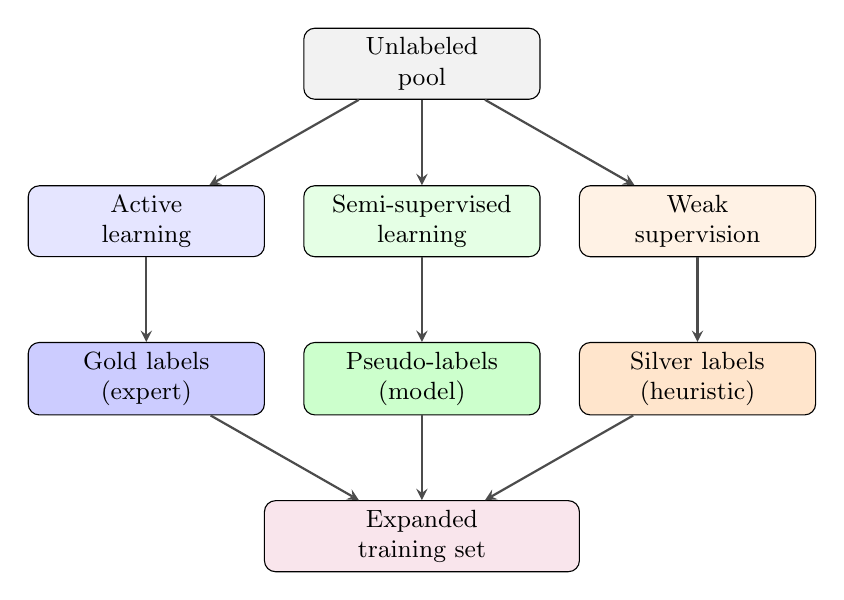
\begin{tikzpicture}[
  x=1cm, y=1cm, font=\small,
  box/.style={draw, rounded corners, minimum height=0.9cm, minimum width=3.0cm, align=center, fill=#1},
  arr/.style={->, >=stealth, thick, black!70}
]
%% Unlabeled pool
\node[box=gray!10] (pool) at (0, 0) {Unlabeled\\pool};

%% Three strategies
\node[box=blue!10] (active) at (-3.5, -2.0) {Active\\learning};
\node[box=green!10] (semi) at (0, -2.0) {Semi-supervised\\learning};
\node[box=orange!10] (weak) at (3.5, -2.0) {Weak\\supervision};

%% Label types
\node[box=blue!20] (gold) at (-3.5, -4.0) {Gold labels\\(expert)};
\node[box=green!20] (pseudo) at (0, -4.0) {Pseudo-labels\\(model)};
\node[box=orange!20] (silver) at (3.5, -4.0) {Silver labels\\(heuristic)};

%% Training set
\node[box=purple!10, minimum width=4.0cm] (train) at (0, -6.0) {Expanded\\training set};

%% Arrows
\draw[arr] (pool) -- (active);
\draw[arr] (pool) -- (semi);
\draw[arr] (pool) -- (weak);
\draw[arr] (active) -- (gold);
\draw[arr] (semi) -- (pseudo);
\draw[arr] (weak) -- (silver);
\draw[arr] (gold) -- (train);
\draw[arr] (pseudo) -- (train);
\draw[arr] (silver) -- (train);
\end{tikzpicture}%
}
\caption{Three complementary strategies for expanding a training set from a large unlabeled pool. Active learning produces gold labels through strategic expert annotation. Semi-supervised learning produces pseudo-labels from model confidence. Weak supervision produces silver labels from heuristics and rules.}
\label{fig:label-acquisition-pipeline}
\end{figure}

\textbf{Label-acquisition strategy.} Before building a model, ask the cheapest way to get labels that are good enough. If expert labels are cheap, label everything. If they are expensive, design a pipeline that combines cheap silver labels for coverage with strategic gold labels for quality. The label-acquisition strategy is as important as the model architecture.

\section{Data Augmentation as a Modeling Decision}

Data augmentation generates new training examples from existing ones by applying transformations. Every augmentation encodes a claim: the model should be invariant to this transformation.

\subsection{Augmentation by Modality}

\textbf{Text augmentation.} Common techniques:
\begin{itemize}[leftmargin=*]
\item \emph{Paraphrase}: rewrite a sentence to mean the same thing (e.g., ``the student is struggling'' $\to$ ``the student is having difficulty'')
\item \emph{Back-translation}: translate to another language and back to introduce variation (e.g., English $\to$ French $\to$ English)
\item \emph{Token replacement}: replace words with synonyms or similar words
\item \emph{Cutoff and mixup}: remove or interpolate between texts
\end{itemize}

For the course-support system, augmentation could paraphrase student messages to simulate the same underlying intent phrased differently.

\textbf{Vision augmentation.} Common techniques:
\begin{itemize}[leftmargin=*]
\item \emph{Rotation, crop, and flip}: rotate or flip the image; crop to different regions
\item \emph{Brightness, contrast, hue adjustment}: vary lighting and color
\item \emph{Noise injection}: add random noise
\item \emph{Geometric transformation}: apply affine or perspective transformations
\end{itemize}

For the pedestrian detector, rotation and brightness adjustment make sense because pedestrians can appear in different lighting and at different angles. Flipping may also be appropriate: the model should detect pedestrians facing left or right equally well.

\textbf{Tabular augmentation.} Techniques like SMOTE (Synthetic Minority Over-sampling Technique) generate synthetic minority examples by interpolating between existing ones. Simpler approaches include adding noise, permuting values, or other local perturbations.

\subsection{Augmentation Risks}

Not every transformation is valid for every task. An augmentation is valid only if the true label is preserved under the transformation.

\begin{warningbox}
Consider a student-message classifier that predicts whether a message indicates urgent need. Paraphrasing is a valid augmentation: ``I missed the deadline'' and ``I couldn't meet the deadline'' should share a label. Cutoff (removing portions of the text) may not be valid: removing the word ``suicide'' from a longer message changes what the message is. Be explicit about which augmentations preserve task semantics.
\end{warningbox}

\begin{example}[Augmentation Mistakes]
A team building a sentiment-analysis model for student feedback augments training texts by removing punctuation and shortening them. Sentences like ``I hate this---the worst!'' become ``I hate this the worst,'' which still conveys negative sentiment. But a crude shortening rule can flip meaning: ``The class is not engaging'' becomes ``The class is engaging'' if the augmenter drops short negation words. The team should have inspected augmented examples and verified that sentiment was preserved.
\end{example}

\section{Synthetic Data: Promise and Pitfalls}

Synthetic data is generated rather than observed. It can address data scarcity, privacy constraints, and rare events, but it comes with serious risks.

\subsection{When Synthetic Data Helps}

Synthetic data is valuable for:
\begin{itemize}[leftmargin=*]
\item \emph{Rare events}: if the real data contains very few traffic accidents or security breaches, synthetic data can supplement real examples to help the model learn the pattern
\item \emph{Privacy constraints}: if you cannot share real patient or financial data, synthetic data lets you build models without exposing sensitive information
\item \emph{Cost reduction}: if generating data through simulation is cheap (e.g., rendering images from a game engine) but collecting real data is expensive, synthetic data can reduce labeling costs
\item \emph{Controlled testing}: synthetic data lets you test the model on edge cases and failure modes that would be rare in real data
\end{itemize}

\subsection{When Synthetic Data Misleads}

Synthetic data is risky because it can encode unrealistic assumptions.

\textbf{Distribution mismatch.} Synthetic data generated from a simulation may not match the real-world distribution. A pedestrian detector trained on game-engine renderings may fail on real photographs because textures, lighting, and pose distributions differ. This is the ``sim-to-real'' gap.

\textbf{Mode collapse.} A generative model may produce synthetic data that is too similar, covering only a narrow slice of the possible variation. A generative adversarial network (GAN) might produce only frontal pedestrian poses and miss side views.

\textbf{False confidence.} A model trained entirely on synthetic data may perform well on held-out synthetic test data but fail on real data. Evaluated against synthetic data, the numbers look good; real-world deployment reveals the gap. This is why evaluation discipline is critical: validate synthetic data against real held-out performance, never against itself.

In autonomous-driving research, simulators like CARLA generate training data because real driving data is expensive to collect and label. Simulation studies repeatedly show that transfer depends on how closely the simulator matches the real sensing and control setting \citep{amini2020vista}. Rendered scenes can differ enough from real camera imagery that simulation-trained models fail to transfer unless the gap is measured and managed. Synthetic data is a starting point, not a complete replacement for real data.

Some recent work uses large pretrained generative models to synthesize more realistic training data. The same evaluation discipline applies: validate the synthetic-augmented model on a real held-out test set, not only on synthetic test data. The false-confidence problem persists.

\subsection{Evaluation Discipline for Synthetic Data}

When using synthetic data, enforce these rules:
\begin{itemize}[leftmargin=*]
\item Train and validate on a mix of real and synthetic data when possible.
\item Always hold out a real-data test set; never evaluate only on synthetic test data.
\item Report performance on real and synthetic held-out data separately to expose any gap.
\item Where possible, use domain-adaptation metrics or transfer performance to quantify the mismatch.
\end{itemize}

\begin{decisionbox}
\textbf{Synthetic data decision checklist:}
\begin{itemize}
\item Is real data genuinely scarce or expensive, or could more be collected?
\item Is the synthetic-data generator reliable and realistic, or does it rely on simplifying assumptions?
\item Can you hold out real data for testing, or will you evaluate only on synthetic data?
\item How large a sim-to-real gap is acceptable for your use case?
\item If synthetic test performance is high but real-world performance is poor, what will you do?
\end{itemize}
\end{decisionbox}

\section{The Data Design Card}

A data design card is a structured document that records the data-design choices made when building a dataset. It serves as institutional memory and makes assumptions explicit. It is the chapter artifact.

\subsection{Data Design Card Structure}

\begin{table}[t]
\centering
\small
\setlength{\tabcolsep}{4pt}
\begin{tabular}{@{}L{2.45cm}L{7.55cm}@{}}
\toprule
Card field & What must be documented \\
\midrule
Data source and collection method & Where the data came from, how it was collected, what dates or time periods it covers, and what population it represents \\
Data extent & Total number of examples, splits (train/val/test sizes and dates), and coverage of important subgroups or conditions \\
Labeling protocol and annotators & Who labeled the data, what guidelines they followed, how long training took, and their background or expertise \\
Annotator agreement & Inter-annotator agreement scores (kappa, alpha, or agreement percentage) and any examples of disagreement \\
Known gaps and limitations & What subgroups or conditions are underrepresented, what distribution shifts are known to exist between training and deployment, and what edge cases may be missing \\
Class distribution and imbalance strategy & The class balance in the dataset, how it compares to the deployment distribution, and what strategy was used to handle imbalance (reweighting, resampling, threshold adjustment, etc.) \\
Label-acquisition strategy & Whether labels are gold (expert), silver (weak supervision), or pseudo (self-training); what labeling functions or heuristics were used; what confidence thresholds were applied; and what fraction of training labels come from each source \\
Governance and escalation & Consent or lawful basis, access controls, sensitive attributes, human-review requirement, crisis-escalation protocol, and no-automation boundaries \\
\bottomrule
\end{tabular}
\caption{A data design card documents collection, labeling, coverage, and governance choices so the dataset's assumptions are clear to future users.}
\label{tab:data-design-card}
\end{table}

\begin{table}[t]
\centering
\small
\setlength{\tabcolsep}{4pt}
\begin{tabular}{@{}L{2.45cm}L{7.55cm}@{}}
\toprule
Card field & What must be documented \\
\midrule
Augmentation claims & What augmentations were applied, what transformations they represent, and why those transformations preserve label validity \\
Synthetic data usage & What synthetic data was included, how it was generated, and what real-data validation was performed to confirm sim-to-real performance \\
Noise and cleaning & Estimated label-noise rates, what cleaning or validation was performed, and confidence in label quality \\
Version and refresh plan & The current version, when the data was last updated, how often it will be refreshed, and who owns the dataset \\
\bottomrule
\end{tabular}
\caption{A data design card also records transformation, synthetic-data, cleaning, and maintenance claims that affect downstream trust.}
\label{tab:data-design-card-maintenance}
\end{table}

\subsection{Filled Example: Course-Support Dataset}

\begin{example}[Data Design Card for Student Early Warning]

\textbf{Data source and collection method.} Student messages and submission records from a first-year undergraduate course offered at a large public university in fall semesters 2021--2024. Data collected from the learning management system (Canvas). No additional manual collection beyond the system's normal logging.

\textbf{Data extent.} 12,480 student messages from 840 unique students across four semesters. 7,480 messages from fall 2021--2022 (training), 2,500 messages from fall 2023 (validation), 2,500 from fall 2024 (test). Covers two course sections: in-person (60\%) and hybrid (40\%); all first-year students.

\textbf{Labeling protocol and annotators.} Messages labeled by three trained academic advisors using standardized guidelines. Labels: URGENT (student mentions mental health crisis, financial hardship, or family emergency), CONCERNING (multiple late submissions in one week, sudden engagement drop), ROUTINE (all others). Annotators trained for 4 hours on 50 messages before labeling began.

\textbf{Governance and escalation.} Access is limited to the academic-support team and the data steward. Sensitive personal attributes are excluded from model inputs unless explicitly approved for bias auditing. URGENT labels trigger a human escalation protocol, not an automated decision. Messages indicating immediate danger are routed to the institution's existing crisis-response process regardless of model score. Students are not punished or denied services because of a model output.

\textbf{Annotator agreement.} Fleiss's kappa = 0.72 (substantial agreement). Disagreements most common between ROUTINE and CONCERNING (14\% of examples); disagreements between URGENT and others rare (2\%). URGENT labels rarely disagreed because guidelines are clearest. ROUTINE vs. CONCERNING reflects genuine ambiguity about ``concerning enough to flag.''

\textbf{Known gaps and limitations.} Dataset covers only one institution and one course. No non-native English speakers' data. No messages from summer sessions or condensed courses. Advisor background: two advisors have counseling training, one does not, which may bias URGENT labeling. Advisors may have unconscious bias toward certain student names or demographics.

\textbf{Class distribution.} ROUTINE: 70\% (8,736 examples), CONCERNING: 22\% (2,738), URGENT: 8\% (1,006). Deployment is expected to have similar distribution (advisors report these ratios). No resampling applied; class-weighted loss was used during training to give higher weight to URGENT examples (weight = 3.0) and CONCERNING examples (weight = 1.5).

\textbf{Label-acquisition strategy.} All 12,480 labels are gold (expert-annotated). No semi-supervised or weak supervision methods were used because annotator time was available. However, future versions may use labeling functions (keyword matching for URGENT, engagement metrics for CONCERNING) to generate silver labels for an additional 50,000 unlabeled messages from earlier semesters, with gold evaluation on the existing test set.

\textbf{Augmentation claims.} No augmentation applied. Student messages are real examples; paraphrasing them would risk changing intent or urgency markers.

\textbf{Synthetic data usage.} None. Real student data is available and was deemed preferable to synthetic data.

\textbf{Noise and cleaning.} No automated cleaning applied. Two messages flagged as potential noise: one appeared to be spam and one was a system notification rather than a student message. These were retained in the training set (not enough to worry about) but are documented. Estimated label-error rate: 2\% based on spot-checking.

\textbf{Version and refresh plan.} Version 1.0, created June 2024. Planned refresh annually to include new semester data. Owned by the Academic Support office.

\end{example}

A data design card is not just documentation. It is a forcing function. Writing one exposes gaps in your understanding of the data. If you cannot fill the ``annotator agreement'' field, measure inter-annotator agreement before building a model. If you cannot describe the ``known gaps'' field clearly, investigate the data more carefully.

\section{Common Mistakes in Data Design}

Several mistakes recur when teams build datasets. The first is treating data as fixed and given rather than as a design choice. The second is ignoring annotator agreement or treating disagreement purely as noise. The third is assuming that balancing classes is always right, without considering the deployment distribution. The fourth is collecting synthetic or augmented data without validating against real held-out data. Finally, too many teams build models without documenting data assumptions, leaving others unable to tell what the model was trained on or where it falls short.

\section{Looking Ahead}

This chapter argued that dataset construction is a design choice, not preprocessing---the examples collected, the labels assigned, the imbalance handled or accepted, and the augmentations used all shape what the model can possibly learn.

The next chapter takes that into the training loop: once the dataset is honestly constructed, how do we actually fit a model to it without wasted compute or hidden bias? Chapter~\ref{ch:optimization-neural-networks} treats optimization as a designed process. Two chapters later, Chapter~\ref{ch:probabilistic-models} treats model-family choice as a modeling judgment rather than a model-selection contest: what counts as a defensible probabilistic structure for the task, and where does that judgment come from?

Two chapters later, the same design discipline is pushed into evaluation: even with a well-designed dataset and a defensible model, what evidence justifies the claim the team wants to make about deployment behavior?

\begin{chaptersummary}
\item Datasets are designed objects. The collection plan, the labeling protocol, the class balance, and the augmentations encode claims about the world that the model will inherit and amplify.
\item Inter-annotator agreement and label noise are information, not nuisance. A 65\% kappa is a fact about the task's ambiguity; soft labels, adjudication, or task redefinition are the design responses---never silent averaging.
\item Class balance is a deployment question, not a default. Match the training distribution to the deployment distribution by default; depart from that only when the deployment cost structure or model class requires it, and document the departure.
\item When labels are scarce, the label-acquisition strategy---which examples get gold labels, which get silver labels from heuristics, and which get pseudo-labels from the model itself---is the modeling decision, not the loss function.
\item Active learning, semi-supervised learning, and weak supervision are not interchangeable. They answer different questions: which examples to label next, how to use unlabeled structure, and how to manufacture noisy labels at scale.
\item Augmentation is a label-preserving claim about invariance. Each transformation says ``the label still holds.'' If that claim is wrong, augmentation injects noise faster than it adds signal.
\item Synthetic data is useful only insofar as it has been validated against held-out real data. Without that validation, the sim-to-real gap silently becomes the deployment gap.
\item The data design card is the chapter's artifact. Its job is to make the data assumptions visible so that a future reader can tell what the model was trained on and where it falls short.
\end{chaptersummary}

\begin{studyquestions}
\item Why is dataset construction a modeling decision rather than just preprocessing?
\item When is inter-annotator disagreement information rather than noise?
\item How should the choice between soft labels and hard labels be made?
\item What does asymmetric label noise do to model learning?
\item When is balancing classes the right choice, and when is it wrong?
\item How do you decide whether to invest in more data, better labels, or better coverage?
\item When is active learning valuable, and when is it wasteful?
\item How does self-training amplify a model's existing biases?
\item What is the difference between gold labels, silver labels, and pseudo-labels?
\item Why does the label model in data programming need to estimate correlations between labeling functions?
\item When should you combine active learning with weak supervision?
\item What claim does every data augmentation encode?
\item What is the sim-to-real gap, and why does it matter?
\item Why should synthetic data be validated against real held-out data?
\item What should a data design card accomplish?
\end{studyquestions}

\begin{exercises}
\item \exercisetag{Design}{Core}Write annotation guidelines for either student-support messages or another classification task. Include at least three label categories and guidance on edge cases.
\item \exercisetag{Calculation}{Core}Compute inter-annotator agreement by hand for a small dataset where two annotators labeled the same five examples. Use the simple agreement percentage and discuss what mismatch you observe.
\item \exercisetag{Design}{Core}For a classification task in your domain, sketch what class imbalance looks like and decide whether the training set should match the deployment distribution or be deliberately rebalanced.
\item \exercisetag{Design}{Intermediate}Design an active learning experiment: specify the task, the model that will make uncertainty estimates, and the query strategy (uncertainty, diversity, or expected model change).
\item \exercisetag{Design}{Intermediate}Write five labeling functions for a classification task in your domain (or the course-support running case). For each, state what pattern it detects, what label it assigns, and estimate its precision and coverage.
\item \exercisetag{Design}{Intermediate}Design a self-training experiment: specify the labeled seed size, unlabeled pool size, confidence threshold, and how you would detect confirmation bias. What validation checks would you perform after each round?
\item \exercisetag{Design}{Intermediate}Propose two sensible data augmentations for either text, image, or tabular data in your domain. For each, argue why the augmentation preserves label validity.
\item \exercisetag{Design}{Advanced}Create a data design card (Table~\ref{tab:data-design-card}) for a dataset in a domain you know or have researched. If carrying one case through the book, use the same case as your framing memo and evaluation plan so the three documents can be read together.
\item \exercisetag{Research}{Advanced}For a public dataset like CIFAR-10 or ImageNet, research what label errors or distribution shifts have been documented. Write a paragraph explaining what was found and what impact it had on models trained on that dataset.
\item \exercisetag{Implementation}{Core}Hand-write a tiny corpus of about 30 short messages about a course-support task, with gold labels for two classes (e.g., \texttt{logistics} vs.\ \texttt{content}). Write three labeling functions in Python: one keyword rule, one length-based rule, and one regex rule. Each LF should return $+1$, $-1$, or $0$ (abstain). Combine them by majority vote, breaking ties by abstaining, and compare the precision and coverage of (i) each individual LF and (ii) the majority-vote ensemble against the gold labels. Report a 3-row table; comment on whether the ensemble improved both axes or traded one for the other.
\end{exercises}

\begin{challengeexercises}
\item \exercisetag{Design}{Advanced}A team builds a pedestrian detector trained on mostly clear daytime frames. At deployment, it underperforms at dusk and in rain. Argue whether the problem is likely more data, better labels, or better coverage. What data-design changes would you recommend?
\item \exercisetag{Concept}{Advanced}A dataset has a 90--10 class imbalance. A baseline majority-class classifier achieves 90\% accuracy. The team balances the dataset and trains a model that achieves 75\% accuracy on the balanced training set but 85\% accuracy on the imbalanced test set. Explain this result and argue whether balance was the right choice.
\item \exercisetag{Concept}{Advanced}Suppose you are given student messages labeled by advisors with 65\% inter-annotator agreement (Cohen's kappa). Should you average disagreements into soft labels or adjudicate? Argue both sides.
\item \exercisetag{Concept}{Advanced}A team uses weak supervision to label 100,000 examples with silver labels and trains a model that achieves 88\% accuracy on a gold test set. The same model trained on only 2,000 gold labels achieves 84\% accuracy. A colleague argues that the weak supervision is ``barely better'' and not worth the engineering effort. Evaluate this argument: what factors beyond overall accuracy should inform the decision?
\item \exercisetag{Design}{Advanced}Design a synthetic data experiment for a task where real data is scarce. State how you would generate the synthetic data, what validation you would perform, and how you would measure sim-to-real gap.
\end{challengeexercises}
